% =============================================================================
% Plantilla de POSTER — Laboratorio 4: Capa de Red (OMNeT++)
% Cátedra de Redes y Sistemas Distribuidos — FaMAF/UNC
%
% Tamaño: A0 vertical (84,1 cm × 118,9 cm) — dos columnas.
% Logos: figuras/logos/unc-escudo-famaf.png, figuras/logos/logo-famaf.png
%
% Compilación (desde esta carpeta):
%   pdflatex lab4-poster.tex
%   pdflatex lab4-poster.tex   % segunda pasada recomendada
%
% Requiere la carpeta figuras/logos/ con los archivos indicados abajo.
% =============================================================================

\documentclass[final]{beamer}

\usepackage[size=a0,orientation=portrait,scale=1.14]{beamerposter}
\usepackage[T1]{fontenc}
\usepackage[utf8]{inputenc}
\usepackage{graphicx}
\usepackage{booktabs}
\usepackage{amsmath}
\usepackage{tikz}
\usepackage{pgfplots}
\pgfplotsset{compat=1.18}
\pgfplotsset{
  every axis/.append style={
    tick label style={font=\large},
    label style={font=\Large},
    title style={font=\Large},
    legend style={font=\large},
  }
}
\usetikzlibrary{arrows.meta,calc,positioning,shapes.geometric}

% --- Datos del grupo ------------------------------------------------------------
\newcommand{\TituloPoster}{Routing Strategies for Ring Topologies in}
\newcommand{\TituloPosterLinea}{OMNeT++}

\newcommand{\IntegrantesPoster}{Álvarez, Lis Ailín; Pinilla, Lautaro; Sabino, Lucas}
\newcommand{\GrupoPoster}{Grupo 23}

% --- Logos (descargados de unc.edu.ar y famaf.unc.edu.ar) -----------------------
% Logos: unc-escudo-famaf.png = escudo UNC con fondo #064F63 (encabezado)
\newcommand{\LogoUNC}{figuras/logos/unc-escudo-famaf.png}
\newcommand{\LogoFAMAF}{figuras/logos/logo-famaf.png}

% --- Paleta (armonizada con logo FaMAF #0B8BAB) ---------------------------------
\definecolor{FamafPrimary}{HTML}{0B8BAB}   % color del logo
\definecolor{FamafDark}{HTML}{064F63}      % encabezado y pie
\definecolor{FamafMedium}{HTML}{087A96}    % variantes en gráficos
\definecolor{FamafLight}{HTML}{E8F5F9}     % fondos de bloques
\definecolor{FamafAccent}{HTML}{E8A838}    % acento cálido (alertas, año)
\definecolor{TextDark}{HTML}{2C3E50}
\definecolor{GuideBg}{HTML}{D6EEF5}        % cajas guía

\title{\TituloPoster\\[0.4cm]\TituloPosterLinea}
\author{\IntegrantesPoster}

\newcommand{\guia}[1]{%
  \par\vspace{0.3em}%
  {\normalsize
  \colorbox{GuideBg}{\parbox{0.97\linewidth}{\textcolor{FamafDark}{\textbf{Guía:}}~#1}}%
  }%
  \par\vspace{0.3em}%
}

% --- Estilo beamer --------------------------------------------------------------
\usetheme{default}
\setbeamercolor{headline}{bg=FamafDark,fg=white}
\setbeamercolor{author in head/foot}{bg=FamafDark,fg=white}
\setbeamercolor{block title}{bg=FamafPrimary,fg=white}
\setbeamercolor{block body}{bg=FamafLight,fg=TextDark}
\setbeamercolor{item}{fg=FamafPrimary}
\setbeamercolor{block alerted title}{bg=FamafAccent,fg=white}
\setbeamercolor{block alerted body}{bg=FamafLight,fg=TextDark}

\setbeamerfont{title}{size=\VeryHuge,series=\bfseries}
\setbeamerfont{author}{size=\Large}
\setbeamerfont{block title}{size=\LARGE,series=\bfseries}
\setbeamerfont{block alerted title}{size=\LARGE,series=\bfseries}
\setbeamerfont{block body}{size=\large}
\setbeamerfont{itemize/enumerate body}{size=\large}

% Encabezado (compatible con una sola compilación)
\setbeamertemplate{headline}{%
  \begin{beamercolorbox}[wd=\paperwidth,leftskip=1.6cm,rightskip=1.4cm,sep=0.65cm]{headline}
    \begin{columns}[T,totalwidth=\textwidth]
      \begin{column}{0.13\textwidth}
        \centering
        \includegraphics[height=4.6cm,keepaspectratio]{\LogoUNC}
      \end{column}
      \begin{column}{0.70\textwidth}
        \centering
        {\fontsize{44}{52}\selectfont\bfseries \TituloPoster\par}
        \vspace{0.2cm}
        {\fontsize{52}{58}\selectfont\bfseries\textcolor{FamafPrimary}{\TituloPosterLinea}\par}
        \vspace{0.35cm}
        {\LARGE\textbf{Laboratorio 4 — Capa de Red}\par}
        \vspace{0.55cm}
        {\Large\insertauthor\par}
        \vspace{0.25cm}
        {\large\textcolor{white!92}{\GrupoPoster \ $\bullet$ \ FaMAF/UNC}\par}
      \end{column}
      \begin{column}{0.13\textwidth}
        \centering
        \includegraphics[height=4.3cm,keepaspectratio]{\LogoFAMAF}
      \end{column}
    \end{columns}
  \end{beamercolorbox}
}

% Pie de página
\setbeamertemplate{footline}{%
  \begin{beamercolorbox}[wd=\paperwidth,leftskip=2.5cm,rightskip=2.5cm,sep=0.85cm,dp=1.2ex]{author in head/foot}
    \begin{columns}[T,totalwidth=\textwidth]
      \begin{column}{0.62\textwidth}
      \end{column}
      \begin{column}{0.36\textwidth}
        \raggedleft\Large
        \textcolor{FamafPrimary}{\textbf{FaMAF/UNC}} — Redes y Sist.\ Distribuidos\\
        \textcolor{FamafAccent}{\textbf{2026}}
      \end{column}
    \end{columns}
  \end{beamercolorbox}
}

\setbeamertemplate{navigation symbols}{}

\newcommand{\RingTopology}{%
  \begin{tikzpicture}[
    ring node/.style={
      circle, draw=FamafPrimary, thick, fill=white,
      minimum size=10mm, inner sep=0pt,
      font=\normalsize\bfseries
    },
    fwd link/.style={
      ->, >=Stealth, thick, draw=FamafDark!85!black,
      shorten >=2mm, shorten <=2mm
    },
  ]
    \def\radius{1.7}
    \foreach \i in {0,...,7} {
      \pgfmathsetmacro{\nodeangle}{90 - 45*\i}
      \node[ring node] (n\i) at (\nodeangle:\radius) {\i};
    }
    \draw[gray!35, dashed, line width=0.5pt] (0,0) circle (\radius);
    \foreach \i/\j in {0/1,1/2,2/3,3/4,4/5,5/6,6/7,7/0} {
      \draw[fwd link] (n\i) -- (n\j);
    }
  \end{tikzpicture}
}

\begin{document}
\begin{frame}[t]

\begin{columns}[T,totalwidth=0.98\paperwidth]

% =============================================================================
% COLUMNA IZQUIERDA — contexto, modelo y análisis
% =============================================================================
\begin{column}{0.46\paperwidth}
  %\hspace{2cm}

  \begin{block}{Motivación y objetivos}
    \begin{itemize}
      \item \textbf{Problema:} Congestión severa por rutas asimétricas en la topología de anillo.
      \item \textbf{Baseline:} Reenvío estático y ciego por \texttt{toLnk[0]} (sentido antihorario).
      \item \textbf{Objetivo:} Diseñar un algoritmo autónomo basado en distancia mínima.
      \item \textbf{Herramienta:} Simulación de tráfico en OMNeT++ (demora, saltos, buffers).
    \end{itemize}
  \end{block}

  \vspace{0.45cm}

  \begin{alertblock}{Eficiencia del algoritmo propuesto}
    \textit{Nuestro algoritmo basado en la distancia mínima elimina la congestión estructural del anillo, balanceando la carga y reduciendo la demora media hasta un 83.5\%.}
  \end{alertblock}

  \vspace{0.45cm}

  \begin{block}{Modelo de simulación}
      \centering
      % Usamos la imagen de tu paper en lugar del dibujo en código
      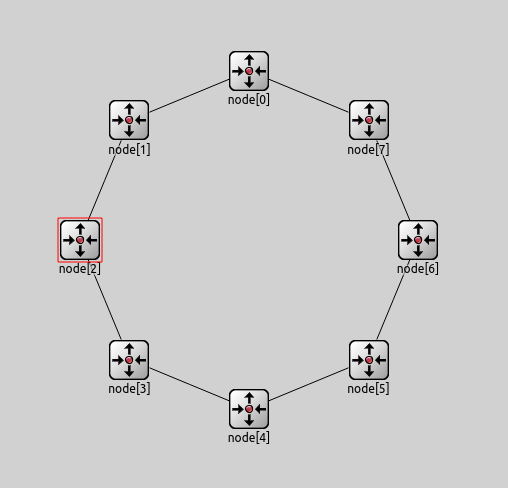
\includegraphics[width=0.75\linewidth]{../paper/figuras/network.png}\\[0.3cm]
      {\Large Topología en anillo — 8 nodos}
      
      \vspace{0.5cm}
      \raggedright
      \textbf{Parámetros Globales (\texttt{omnetpp.ini}):}
      \begin{itemize}
        \item \textbf{Tiempo de simulación:} 200 s \ (\texttt{seed-set = 1})
        \item \textbf{Tamaño de paquete:} 125.000 bytes (1 Mbit)
        \item \textbf{Generación de tráfico:} Exponencial (\texttt{interArrivalTime})
      \end{itemize}
      
      \vspace{0.2cm}
      \textbf{Arquitectura interna:} \texttt{app} $\rightarrow$ \texttt{net} $\rightarrow$ \texttt{lnk[0,1]}\\
      \textbf{Métricas:} Demora E2E, saltos, ocupación de buffer y utilización de enlace.
  \end{block}

  \vspace{0.45cm}

  \begin{block}{Análisis — Caso 1}
    \textbf{Fuentes:} \texttt{node[0]} y \texttt{node[2]} $\rightarrow$ \texttt{node[5]}

    \vspace{0.5cm}
    \centering
    \begin{tikzpicture}
      \begin{axis}[
        width=0.9\linewidth,
        height=5.5cm,
        ybar,
        bar width=12pt,
        ymin=0,
        enlarge x limits=0.12,
        symbolic x coords={Demora,Saltos,Buffer,Enlace},
        xtick=data,
        ylabel={Valor norm.},
        title={Caso 1 — baseline kickstarter},
        legend to name=legCaso1,
        legend style={draw=FamafPrimary!40, fill=white, font=\large},
      ]
        \addplot[fill=FamafDark!75] coordinates {(Demora,0.96) (Saltos,0.60) (Buffer,1.00) (Enlace,1.00)};
        \addplot[fill=FamafPrimary!80] coordinates {(Demora,1.00) (Saltos,1.00) (Buffer,0.11) (Enlace,0.92)};
        \legend{Fuente 0 (atravesando Nodo 0), Fuente 2 (atravesando Nodo 2)}
      \end{axis}
    \end{tikzpicture}

    \vspace{0.35cm}
    \pgfplotslegendfromname{legCaso1}

    \vspace{0.85cm}
    \large
    \renewcommand{\arraystretch}{1.2}
    \begin{tabular}{@{}lrr@{}}
      \toprule
      \textbf{Métrica Global} & \textbf{Prom.} & \textbf{Máx.} \\
      \midrule
      Demora E2E (s) & 53.25 & -- \\
      Saltos         & 3.8  & 5  \\
      Ocupación Buffer (pkts)  & 21.8  & 199 \\
      Utilización Enlace (\%)  & 29.5  & 98.0 \\
      \bottomrule
    \end{tabular}
  \end{block}

  \vspace{0.45cm}


\end{column}

% =============================================================================
% COLUMNA DERECHA — diseño, evaluación y conclusiones
% =============================================================================
\begin{column}{0.46\paperwidth}

    \begin{block}{Análisis — Caso 2}
    \vspace{0.4cm}
    \centering
    \begin{tikzpicture}
      \begin{axis}[
        width=0.9\linewidth,
        height=5.8cm,
        xlabel={\texttt{interArrivalTime} (s)},
        ylabel={Demora media E2E (s)},
        xmin=0, xmax=10,
        xtick={0,2,4,6,8,10},
        ymin=0, ymax=85,
        grid=major,
        title={Estabilidad de la red vs.\ carga ofrecida},
        legend to name=legCaso2,
        legend style={draw=FamafPrimary!40, fill=white, font=\large},
      ]
        \addplot[thick, FamafPrimary, mark=*, mark size=3pt] coordinates {
          (0.5,75.09)(1,65.92)(2,56.52)(4,39.99)(6,17.49)(8,6.19)
        };
        \addlegendentry{Demora E2E Baseline}
        \addplot[thick, FamafAccent, dashed] coordinates {(7,0)(7,85)};
        \addlegendentry{Umbral Saturación (7s)}
      \end{axis}
    \end{tikzpicture}

    \vspace{0.35cm}
    \pgfplotslegendfromname{legCaso2}

    \vspace{0.75cm}
    \raggedright
    \textbf{Cuello de Botella:} \textit{El nodo 6 acumula los 7 flujos de la red. Físicamente inestable para un IAT < 7 segundos.}
  \end{block}

  \begin{block}{Algoritmo propuesto}
    \begin{itemize}
      \item \textbf{Descubrimiento:} Utiliza paquetes de control \texttt{hello}/\texttt{echo} para conocer dinámicamente el tamaño de la topología ($N$).
      \item \textbf{Cálculo:} Evalúa la distancia matemática en ambos sentidos del anillo.
      \item \textbf{Balanceo:} Decide sobre la marcha la interfaz óptima por paquete.
    \end{itemize}
    \vspace{0.3cm}
    {\Large\ttfamily
    horario = (destino - mi\_id + N) \% N\\[0.12cm]
    antihorario = (mi\_id - destino + N) \% N\\[0.12cm]
    si horario $\le$ antihorario:\\[0.12cm]
    \quad enviar por lnk[1] (sentido horario)\\[0.12cm]
    sino:\\[0.12cm]
    \quad enviar por lnk[0] (sentido antihorario)
    }
    \vspace{0.3cm}
    \textbf{Ventaja:} Autónomo. No requiere configurar constantes a mano ni utilizar iteradores trampa como \texttt{cTopology}.
  \end{block}

  \vspace{0.45cm}

  \begin{block}{Evaluación comparativa}

    \vspace{0.4cm}
    \centering
    \begin{tikzpicture}
      \begin{axis}[
        width=0.9\linewidth,
        height=5.8cm,
        ybar,
        bar width=14pt,
        ymin=0,
        enlarge x limits=0.12,
        symbolic x coords={C1-Dem,C1-Sal,C2-Dem,C2-Buf},
        xtick=data,
        x tick label style={rotate=12,anchor=east},
        ylabel={Mejora Normalizada},
        title={Comparativa de Desempeño},
        legend to name=legComp,
        legend style={draw=FamafPrimary!40, fill=white, font=\large},
      ]
        \addplot[fill=FamafDark!75] coordinates {(C1-Dem,1.00) (C1-Sal,1.00) (C2-Dem,1.00) (C2-Buf,1.00)};
        \addplot[fill=FamafPrimary!80] coordinates {(C1-Dem,0.25) (C1-Sal,0.79) (C2-Dem,0.16) (C2-Buf,0.16)};
        \legend{Kickstarter, Algoritmo Propuesto}
      \end{axis}
    \end{tikzpicture}

    \vspace{0.35cm}
    \pgfplotslegendfromname{legComp}

    \vspace{0.75cm}
    \begin{columns}[T,totalwidth=\linewidth]
      \begin{column}{0.48\linewidth}
        \textbf{Mejoras Caso 1:}
        \begin{itemize}
          \item Demora E2E: \textbf{$-74.4\%$}
          \item Buffer Máximo: \textbf{$-86.4\%$}
        \end{itemize}
      \end{column}
      \begin{column}{0.48\linewidth}
        \textbf{Mejoras Caso 2 (IAT=4s):}
        \begin{itemize}
          \item Demora E2E: \textbf{$-83.5\%$}
          \item Buffer Máximo: \textbf{$-84.0\%$}
        \end{itemize}
      \end{column}
    \end{columns}
\vspace{0.35cm}
    \begin{itemize}
      \item \textbf{Bucles de enrutamiento:} Nulos. El paquete viaja de forma monótona acercándose al destino, limitando el máximo a 4 saltos.
      \item \textbf{Umbral teórico de estabilidad:} mejorado de 7s a 4s al reducir la concentración máxima de 7 a 4 flujos.
    \end{itemize}
  \end{block}

  \vspace{0.45cm}

  \begin{alertblock}{Conclusiones}
    \begin{itemize}
      \item El algoritmo kickstarter concentra el tráfico asimétricamente, generando un severo \textit{queueing delay} al forzar 7 flujos a transitar por un mismo nodo, colapsando con cargas medias.
      \item Nuestra estrategia distribuye los flujos en ambos sentidos del anillo. Esto reduce dramáticamente la demora y aleja el umbral de estabilidad teórico de 7s a 4s, permitiendo a la red procesar de forma completamente estable intervalos de llegada (IAT) de 6s que antes colapsaban la red.
      \item \textbf{Trabajo futuro:} Implementar mensajes \emph{keepalive} periódicos en reemplazo del \emph{hello} inicial para detectar la caída de nodos y dotar a la red de tolerancia a fallos.
    \end{itemize}
  \end{alertblock}


\end{column}

\end{columns}

\end{frame}
\end{document}
